\part{Machine Learning, Deep Learning y el concepto de anomalía}
\label{part:machine_learning_deep_learning_anomalia}

\chapter{Concepto de Anomalía y Series Temporales}
\label{chapter:anomalia}

\section{Concepto de Anomalía}

Debemos de tener en cuenta que el concepto de anomalía no es algo fácil de definir. Tanto es así que, por ligeros cambios o matices en la definición, podemos estar cayendo en un concepto completamente distinto.

Antes de comenzar debemos aclarar el objetivo que vamos persiguiendo, es decir, el concepto de anomalía que nos va a interesar. Podemos encontrar muchas definiciones de anomalías, pero en nuestro caso nos vamos a centrar en la dada por Carreño, Inza y Lozano en \cite{ander_analyzing_2019}.

Según estos autores podemos definir el contexto de la detección de anomalías en 4 subtipos: eventos raros, anomalías, novedades y outliers. 

En primer lugar, tenemos los eventos raros. Tenemos un problema en el que hay un tipo de datos que aparecen con muy poca frecuencia en el contexto de las series temporales y queremos detectar dicho tipo de eventos. Estamos en una perspectiva supervisada, por lo que esto no es más que un problema de clasificación altamente desbalanceado en el contexto de las series temporales. En este escenario el problema se resuelve aplicando distintas técnicas que favorezcan que los clasificadores aprendan bien esta clase rara y se detecte. Claramente no es nuestro caso pues no disponemos de etiquetas claras y no es un problema de clasificación.

En segundo lugar tenemos las anomalías. Según Carreño, las anomalías están enmarcadas en conjuntos de datos estáticos. Este simple hecho ya saca el subtipo de nuestro marco de trabajo, pero aún así es bueno ver su definición. Las anomalías son, para Carreño et al., un problema de clasificación altamente desbalanceado en el contexto de datos estáticos. Esto es análogo al caso anterior, salvando el paso de datos estáticos a dinámicos. Claramente no es nuestro caso pues el problema no es de clasificación ni tenemos etiquetas claras ni son datos estáticos de los que disponemos.

En tercer lugar tenemos las novedades. Este apartado puede ser aplicado tanto a datos estáticos como a datos dinámicos. En los dos casos anteriores tenemos problemas de clasificación, pero disponemos de las etiquetas y de ejemplos de todas las clases para la fase de entrenamiento. En las novedades tenemos datos normales de una sola clase en la fase de entrenamiento, por lo que en el momento de entrenar tendremos que definir las fronteras de la única clase que tenemos. El objetivo en este problema es detectar la novedad, es decir, los nuevos ejemplos que no cuadran dentro de la frontera de decisión de la única clase que tenemos en la fase de entrenamiento en el problema. De nuevo esto no es nuestro caso, porque no tenemos etiquetas de los datos normales y por tanto no podemos definir claramente ese marco de trabajo ``one class''.

Por último tenemos los outliers. Este término no es de fácil traducción al español, por lo que es preferible dejar el original en inglés. Este punto engloba la clasificación no supervisada, es decir, tenemos ciertas nociones del conjunto de datos pero ninguna etiqueta precisa y aun así queremos saber qué datos son normales y cuáles anómalos basándonos en alguna técnica que no emplee más que los propios datos sin etiquetar. Este es nuestro marco de trabajo, pues no disponemos de etiquetas claras ni ``ground truth'', oráculo o verdad absoluta a la que recurrir para aprender de ella. Tenemos que elaborar un sistema capaz de detectar los mantenimientos de nuestra máquina sin poder aprender a priori lo que es normal y lo que es anómalo.

Dentro de este esquema de posibilidades ya hemos localizado la que más se acerca al objetivo que queremos cumplir. Como hemos podido ver, es la única opción completamente no supervisada que Carreño contempla en el artículo, lo que nos deja con el escenario más complejo de todos. 

Pensemos un momento todas las posibles definiciones de anomalías que tenemos mediante varios ejemplos.

\begin{figure}[H]
	\centering
	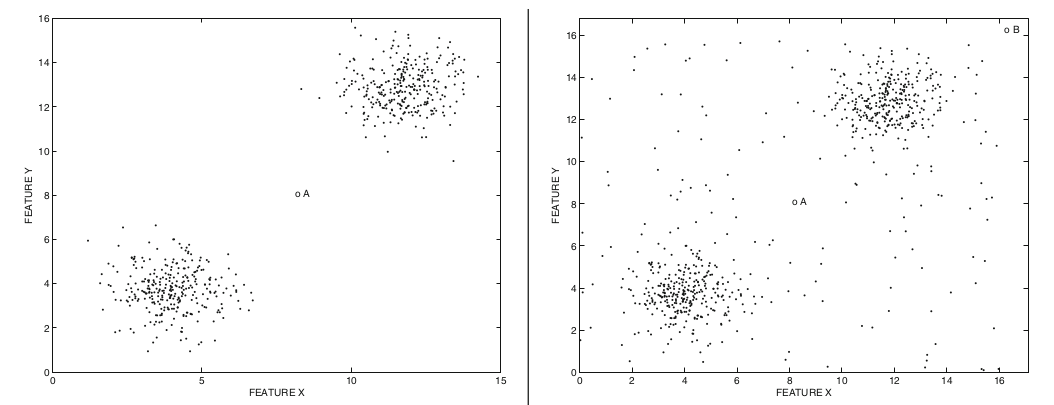
\includegraphics[scale=0.35]{imagenes/ejemplo1_anomalia.png}
	\caption{Ejemplo sin ruido y con ruido de una anomalía. \cite[p21]{aggarwal_outlier_2017}}
	\label{img:ejemplo1-anomalia}
\end{figure}

Como podemos ver, el caso de la izquierda es relativamente fácil de detectar, por ejemplo con un algoritmo de clustering. El ejemplo de la derecha es muchísimo más complejo. En el ejemplo tenemos identificado el mismo punto como anomalía, pero ahora está rodeado de ruido que hace muy complicado detectarlo. Además surge la pregunta de cuándo tenemos ruido y cuándo son puntos anómalos ya que la diferencia en algunos casos es inapreciable.

Para todas estas cuestiones no hay una respuesta que siempre sea la adecuada, pues dependen del contexto en el que estemos y de lo que queramos detectar y hacer con las anomalías. Los algoritmos de detección de anomalías, al no ser fácil la tarea de clasificación por ser no supervisado, nos suelen arrojar un número que puntúa cada instancia. Cuanto mayor sea el número asignado a una instancia mayor es su grado de anomalía. Este sistema nos permite asignar algún tipo de regla que detecte los puntos más anómalos y deje fuera los puntos de los que no estemos seguros. Por tanto, un algoritmo de detección de anomalías por si solo para este problema no es de utilidad. Hay que acompañarlo de un sistema que decida sobre los scores qué puntos son anómalos y cuales no, además de que en nuestro problema no tenemos datos estáticos, si no series temporales, por lo que debemos también dotar de esa temporalidad a las anomalías.

Todos estos aspectos los discutiremos más a fondo cuando nos acerquemos a la sección de experimentación, donde podremos ver mejor la forma final de detectar anomalías y mantenimientos en nuestro caso.

\subsection{Concepto clásico de anomalía}

Vamos a dar una breve definición del concepto clásico de anomalía basado en distancias. Este apartado está basado en el libro Outlier Analysis \cite{aggarwal_outlier_2017}.

La definición clásica comienza en espacios de una única dimensión para poder entender bien el concepto antes de generalizarlo. Si tenemos un espacio de valores reales, solemos aplicar lo que se conoce como el criterio de Tukey. Este criterio nos dice que, si el valor de un punto se sale del intervalo $[Q_1 - k(Q_3 - Q_1), Q_3 + k(Q_3 - Q_1)]$, donde $Q_i$ representan los cuartiles y $k$ es un número arbitrario (normalmente $1.5$, $3$ o $5$), entonces dicho punto es una anomalía.

Este criterio es una primera aproximación simple y únicamente interesante en una dimensión. Podemos intentar extender este mismo criterio haciendo esta comprobación sobre todas las dimensiones o características de nuestros datos, pero esta es una extensión demasiado simple. Esto es fácilmente comprobable con un ejemplo en dos dimensiones:

\begin{figure}[H]
	\centering
	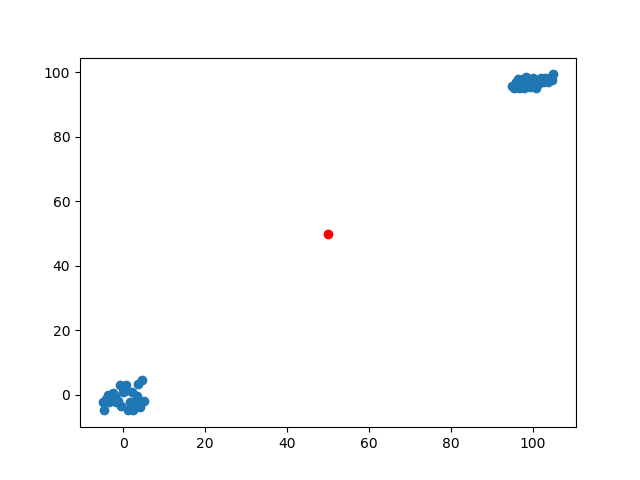
\includegraphics[scale=0.5]{imagenes/outlier_cluster.png}
	\caption{Ejemplo de anomalía entre clusters.}
	\label{img:outlier-cluster}
\end{figure}

Tenemos un punto entre dos cluster en dos dimensiones. Este comportamiento es claramente anómalo pues no entra dentro de ninguno de los clusters ni está cerca aunque esté a medio camino entre los dos, por lo que tenemos una anomalía escondida entre los dos grupos que consideramos normales. Si aplicamos el criterio de Tukey en las dos dimensiones el punto anómalo cae dentro del intervalo normal con mucha holgura. Es por esto que el criterio de Tukey extendiéndolo a todas las dimensiones no es un criterio útil.

Podemos dar un criterio mejor para más dimensiones, por ejemplo podemos agrupar los datos por clusters y calcular la mayor distancia dentro de cada uno de ellos. Si tenemos un punto que se distancie más de $k$ veces dicha distancia máxima de todos los clusters entonces estamos ante una anomalía, pues se distancia de todos los comportamientos normales.

Recordemos que esto no es más que una serie de criterios, que pueden no ser de utilidad para todos los problemas. Por ello debemos de estudiar siempre las peculiaridades de nuestros problemas antes de decidir el algoritmo o criterio que nos puede ayudar más en la detección de anomalías.

\section{Series Temporales}

Ya hemos comentado que vamos a trabajar con series temporales, por lo que antes de empezar cabe definir formalmente lo que consideramos una serie temporal.

Una serie temporal podemos definirla como un par $(t,x)\in \mathbb{R}\times \mathbb{R}$ donde $t$ es un sello temporal, es decir, una cuantificación numérica para el tiempo desde un punto de referencia y $x$ es un valor numérico asociado al valor temporal. De esta forma lo que tenemos son valores numéricos para cada valor temporal.

Si extendemos este concepto podemos definirlo como $(t,x)\in \mathbb{R}\times \mathbb{R}^n$ donde $n$ es la dimensionalidad de la serie temporal, es decir, ahora no toma valores reales si no vectores de valores reales.

Las series temporales se pueden dividir en varias componentes. Esta división tiene la intención de poder entender mejor el comportamiento de la serie, tanto para su estudio como el posterior modelado y predicción si nos interesase.

Las componentes que podemos extraer de una serie temporal son:

\begin{itemize}
	\item Tendencia: nos indica la componente que se mantiene estable a lo largo de toda la serie temporal, por ejemplo podemos tener tendencias crecientes, decrecientes o no tener tendencia en nuestra serie.
	\item Componente estacional: es la componente cíclica que se repite con periodos menores a un año, por ejemplo puede ser por estaciones, meses, semanas u otra fracción de tiempo significativa para el problema.
	\item Componente cíclica: es la componente que recoge los fenómenos periódicos de frecuencia mayor a un año, normalmente de periodo irregular influida por movimientos a menudo dependientes de la tendencia.
	\item Componente residual: es la componente que depende del ambiente del sistema. No tiene ningún tipo de regularidad y podemos decir que depende de las anomalías que se presenten en la serie de forma más común o frecuente.
	\item Componente accidental: esta componente recoge las variaciones que se producen por fenómenos muy raros y aislados.
\end{itemize}

Podemos poner un ejemplo para ilustrar las componentes de una serie. Por ejemplo si tenemos una serie temporal con las temperatura de la tierra actualmente podemos apreciar una tendencia creciente por el cambio climático, por lo que la componente de la tendencia sería creciente. Tenemos una componente estacional que podemos apreciar por las estaciones del año, momentos en los cuales las temperaturas bajan y suben siempre de la misma forma o muy similar. La componente cíclica puede ser por ejemplo las edades de la Tierra, momentos en los cuales las temperaturas bajan y suben dependiendo de las glaciaciones y la flora y fauna de la Tierra. En la componente residual podemos tener por ejemplo fenómenos como tormentas, inundaciones o fenómenos producidos por el hombre. En la componente accidental tendríamos fenómenos mucho más súbitos y repentinos, por ejemplo podríamos poner en esta componente la caída de un meteorito, fenómeno que raramente puede producirse más de una vez o dos.

Visto esto, ya tenemos una idea de lo que vamos a ir buscando y el tipo de datos con los que vamos a tratar. En nuestra serie temporal nosotros nos vamos a preocupar por la componente residual y la accidental, ya que son las componentes en las que se esconden los fenómenos que no son modelables y por tanto escapan al comportamiento normal de las variables.